%1.5.1
%50/50, k = 10 -> tid vs DPI!
%confusion matrix på 1 run (100, 200 og 300 DPI) 
%1.5.2
%k vs Train Size (10 runs)
%1.5.3
%cross val. 10 runs 90/10 -> mean + var


\subsection{Single Person Tests}
This section tests the K-NN algorithm using data from one single person, namely group three member two's data.
%
%The tests are performed first with the data split equally into a 50\% for the training and 50\% for the test set and the runtime is measured and compared for the three different image qualities. 
%
%Then test are performed with changing values of k and the training set size.
%
%Afterwards with a 90/10\% split for training and test respectively is computed and mean and variance is given.
%
%All the tests will be conducted using cross validation with 10 runs.

\subsubsection{Equally Sized Training and Test Set}
To test the algorithm the data from the three different DPI's where split 50/50\% into a training and test set. 
The time to compute the test set for each DPI was then recorded and plotted. This is seen in figure \ref{fig:PersonDependent_5050}.
As expected does this scale with number of pixels. 

% % % % generated by timing.R
\begin{figure}[h]
\centering
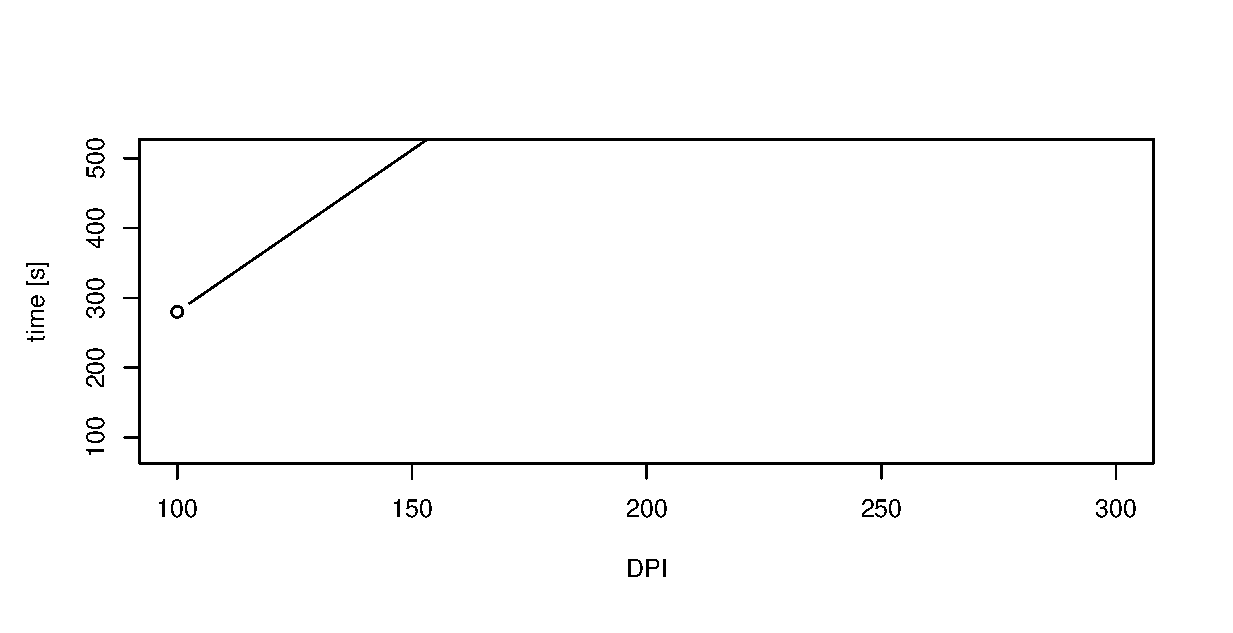
\includegraphics[width=\textwidth]{graphics/time_vs_dpi}
\caption{Timing of running a result with a 50/50\% split of group three member two's data.}
\label{fig:PersonDependent_5050}
\end{figure}

Running the three test sets resulted in the confusion matrices seen in table \ref{tb:confus}.
They are all tested with a K of 10 and a split of 50/50\%.
In these it is seen which numbers do well, which numbers are hard to detect and which number they are detected as.
While the chance of predicting a one when the actual is a one is really high, there seem to be a high chance of predicting a one, when it is not. 
In the case of table \ref{tab:confus_300} only 200 out of the 440 predicted ones were actual ones.
While the overall detection is good, the eights are, with at most 57\% correct predictions, the most difficult to predict correctly. 
This is, as seen in figure \ref{tb:confus}, due to the eights apparent similarity to the ones, threes and nines.


% % % % generated by confusion.R
\begin{table}[H]
    \centering
    \begin{subtable}{0.5\textwidth}
        \flushright
        
\begin{tikzpicture}
            \node at (0,0) {};
            \node at (1,0) {\huge Actual Class}; 
        \end{tikzpicture}
    \end{subtable}

    \begin{subtable}{0.1\textwidth}
        \flushright
        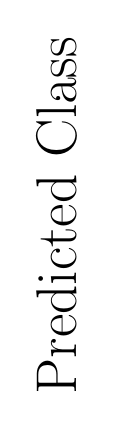
\begin{tikzpicture}
            \node[rotate=90] {\huge Predicted Class};
        \end{tikzpicture}
    \end{subtable}
    \begin{subtable}{0.6\textwidth}
        \begin{subtable}{\textwidth}
            \centering
            {\scriptsize
                \begin{tabular}{l|*{10}{c}}
                    &0	& 1	& 2	& 3	& 4	& 5	& 6	& 7	& 8	& 9 \\
\hline
0	& 172	& 0	& 0	& 0	& 2	& 2	& 5	& 0	& 0	& 0 \\
1	& 18	& 199	& 24	& 21	& 30	& 26	& 25	& 19	& 32	& 57 \\
2	& 2	& 0	& 147	& 3	& 1	& 3	& 2	& 3	& 4	& 1 \\
3	& 5	& 1	& 14	& 172	& 0	& 6	& 18	& 6	& 34	& 14 \\
4	& 0	& 0	& 0	& 0	& 159	& 4	& 1	& 2	& 1	& 20 \\
5	& 0	& 0	& 0	& 0	& 0	& 154	& 0	& 0	& 2	& 0 \\
6	& 1	& 0	& 0	& 1	& 0	& 1	& 149	& 0	& 1	& 0 \\
7	& 0	& 0	& 10	& 2	& 0	& 0	& 0	& 169	& 0	& 1 \\
8	& 0	& 0	& 4	& 0	& 0	& 4	& 0	& 1	& 106	& 5 \\
9	& 2	& 0	& 1	& 1	& 8	& 0	& 0	& 0	& 20	& 102 \\

                \end{tabular}
            }
            \caption{Results for 100 DPI.}
            \label{tab:confus_100}
        \end{subtable}
        \\
        \begin{subtable}{\textwidth}
        \vspace{0.4cm}
            \centering
            {\scriptsize
                \begin{tabular}{l|*{10}{c}}
                    &0	& 1	& 2	& 3	& 4	& 5	& 6	& 7	& 8	& 9 \\
\hline
0	& 172	& 0	& 0	& 0	& 1	& 3	& 0	& 0	& 1	& 1 \\
1	& 26	& 200	& 18	& 37	& 23	& 11	& 24	& 16	& 39	& 58 \\
2	& 0	& 0	& 160	& 2	& 0	& 1	& 4	& 0	& 2	& 0 \\
3	& 0	& 0	& 7	& 155	& 0	& 1	& 20	& 1	& 20	& 16 \\
4	& 0	& 0	& 0	& 0	& 168	& 1	& 0	& 1	& 0	& 6 \\
5	& 0	& 0	& 0	& 0	& 0	& 181	& 1	& 0	& 1	& 0 \\
6	& 2	& 0	& 0	& 0	& 1	& 0	& 150	& 0	& 4	& 0 \\
7	& 0	& 0	& 13	& 5	& 0	& 0	& 1	& 182	& 1	& 2 \\
8	& 0	& 0	& 1	& 0	& 0	& 1	& 0	& 0	& 103	& 1 \\
9	& 0	& 0	& 1	& 1	& 7	& 1	& 0	& 0	& 29	& 116 \\

                \end{tabular}
            }
            \caption{Results for 200 DPI.}
            \label{tab:confus_200}
        \end{subtable}
        \begin{subtable}{\textwidth}
        \vspace{0.4cm}
            \centering
            {\scriptsize
                \begin{tabular}{l|*{10}{c}}
                    &0	& 1	& 2	& 3	& 4	& 5	& 6	& 7	& 8	& 9 \\
\hline
0	& 157	& 0	& 0	& 0	& 1	& 4	& 2	& 0	& 0	& 0 \\
1	& 37	& 200	& 24	& 33	& 17	& 14	& 18	& 19	& 30	& 48 \\
2	& 1	& 0	& 160	& 0	& 0	& 0	& 2	& 0	& 2	& 0 \\
3	& 1	& 0	& 1	& 152	& 0	& 0	& 7	& 1	& 15	& 9 \\
4	& 0	& 0	& 0	& 0	& 179	& 0	& 0	& 0	& 2	& 5 \\
5	& 0	& 0	& 0	& 0	& 1	& 181	& 0	& 0	& 1	& 0 \\
6	& 4	& 0	& 0	& 0	& 1	& 0	& 162	& 0	& 2	& 0 \\
7	& 0	& 0	& 15	& 15	& 0	& 0	& 9	& 180	& 3	& 2 \\
8	& 0	& 0	& 0	& 0	& 0	& 1	& 0	& 0	& 114	& 0 \\
9	& 0	& 0	& 0	& 0	& 1	& 0	& 0	& 0	& 31	& 136 \\

                \end{tabular}
            }
            \caption{Results for 300 DPI.}
            \label{tab:confus_300}
        \end{subtable}
    \end{subtable}
    \caption{Confusion matrices with different picture resolutions.}
    \label{tb:confus}
\end{table}


\subsubsection{Changing K and Training Set Size}
Tests was performed to see how both the value of K and size of the training set affects the accuracy of the K-NN algorithm. 
The result is given in figure \ref{fig:personDependent_contour}.

% \begin{figure}[H]
% \centering
% 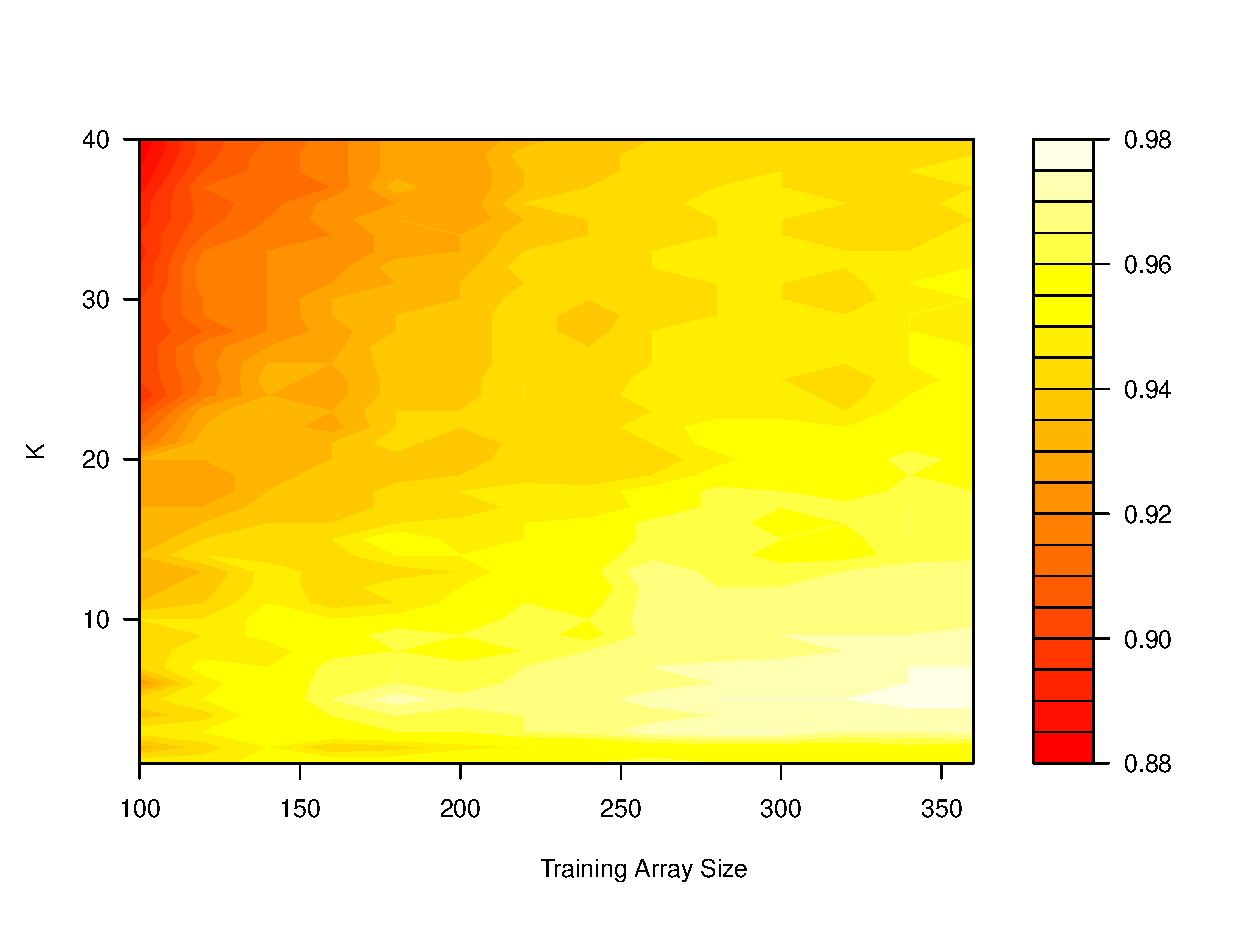
\includegraphics[width = 13cm]{graphics/graph_G3M2_20}
% \caption{Success Rate of the K-NN algorithm for changing values of K and the training set size.}
% \label{fig:personDependent_contour}
% \end{figure}

\begin{figure}[H]
\centering
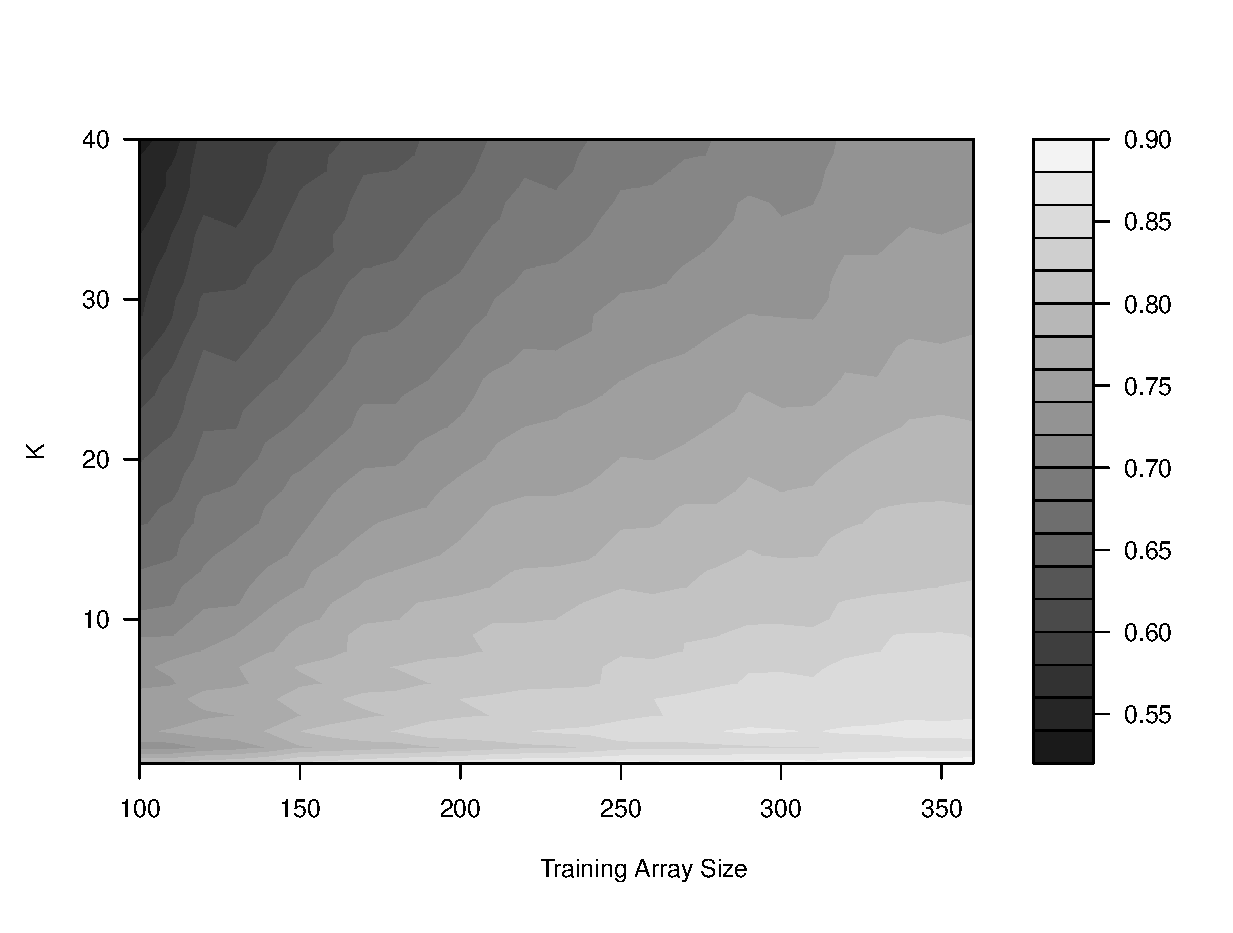
\includegraphics[width = \textwidth]{graphics/graph_G3M2_10_10}
\caption{Success Rate of the K-NN algorithm for changing values of K and the training set size.}
\label{fig:personDependent_contour}
\end{figure}

% \begin{figure}[H]
% \centering
% 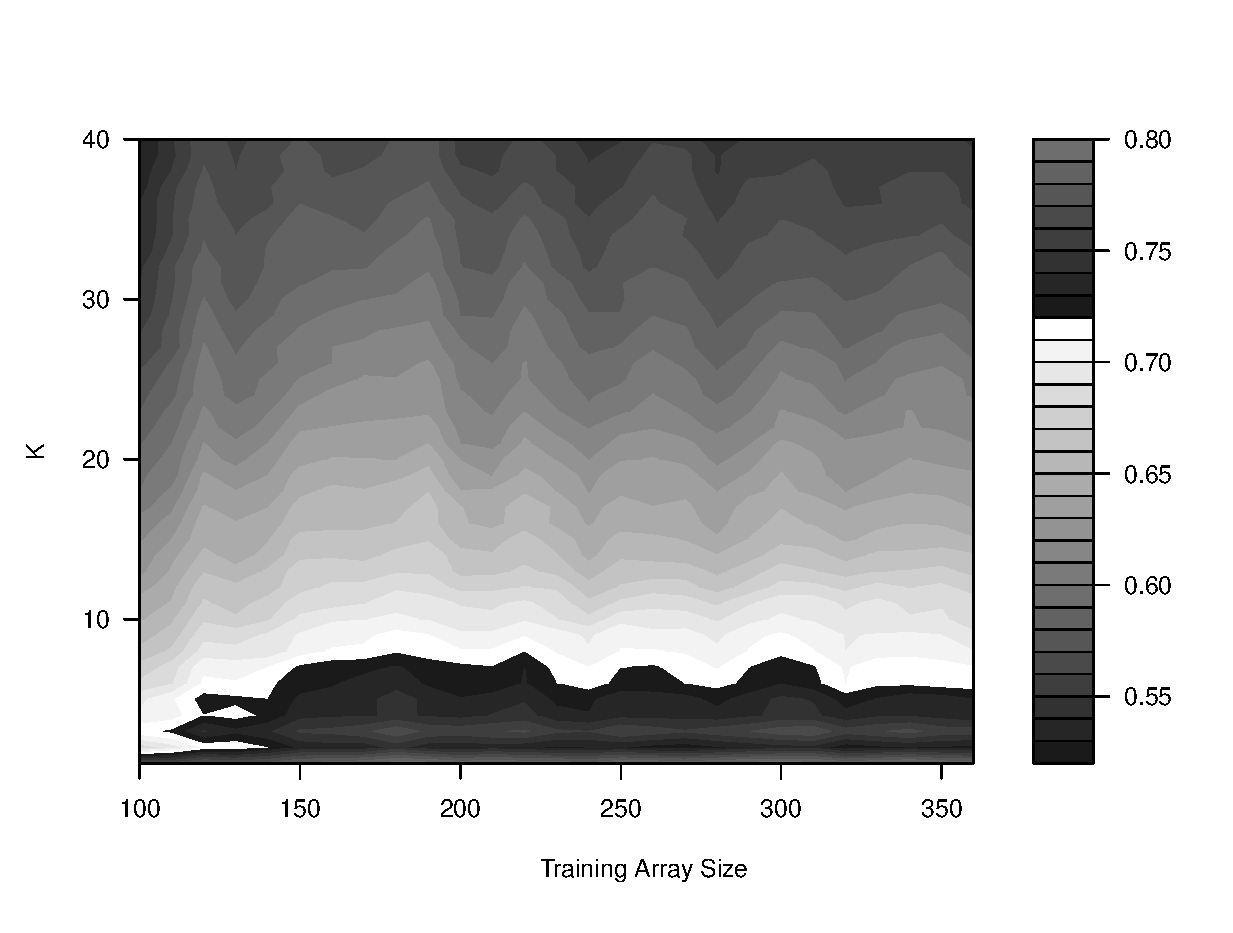
\includegraphics[width = 13cm]{graphics/graph_G3M1_10_10}
% \caption{Success Rate of the K-NN algorithm for changing values of K and the training set size.}
% \label{fig:personDependent_contour}
% \end{figure}

The test conducted in figure \ref{fig:personDependent_contour} where done with a test size of 40 and run 10 times with cross validation.

As seen on figure \ref{fig:personDependent_contour}, then the accuracy of the algorithm appears to increase as the train set size increases.
Furthermore the optimal value of K is dependent on the size of training set. 
As the size of the training set increases, so does the range in which the best performance is obtained.
From figure \ref{fig:personDependent_contour} it can be seen that the results are best when using a training size which is above 300 and K ranging between 2 and 4, but a K of up to 10 can also be used to obtain a decent performance.


\subsubsection{90/10 Data Split}
A cross validation was also carried out using a 90/10\% and 50/50\% split of the data. 
Each test was made on both group members to see the difference.
The result of this is seen in figure \ref{fig:PersonDependent_9010}.
The values can be seen in table \ref{tb:cross}

% % % % Generating this with cross_test.R tonight
\begin{figure}[h]
\centering
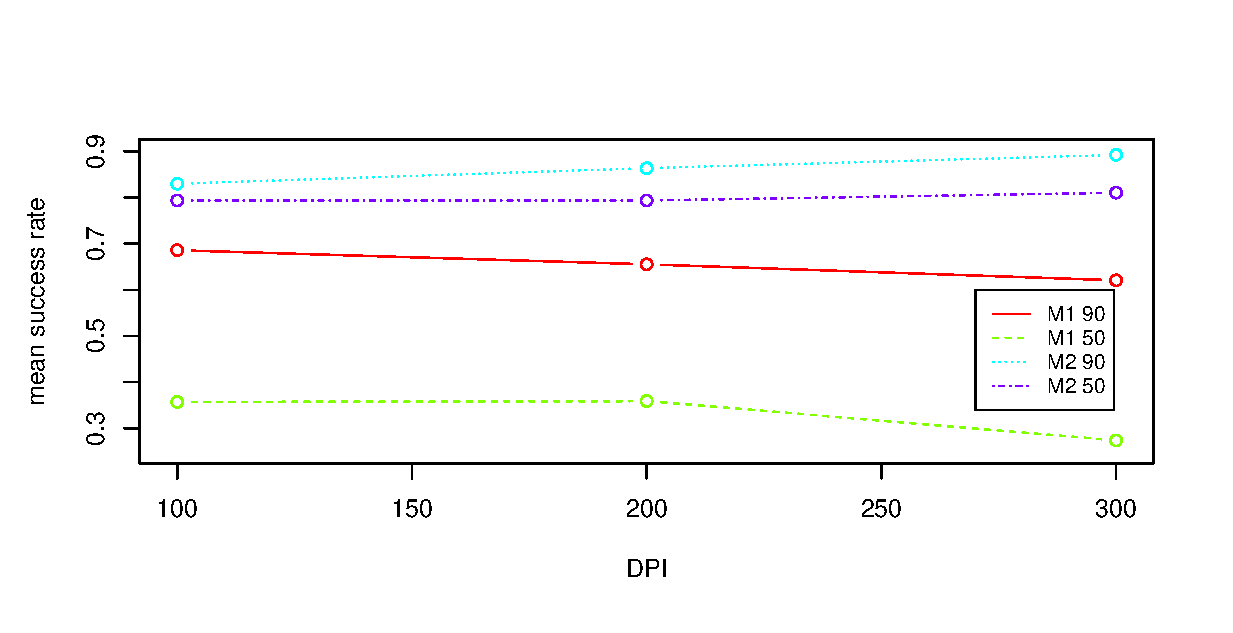
\includegraphics[width=\textwidth]{graphics/cross_test}
\caption[Cross validation]{Test result with a 90/10\% and 50/50\% split. The data points are taken as the mean of 10 runs using cross validation.}
\label{fig:PersonDependent_9010}
\end{figure}

\begin{table}[h]
\centering
    \begin{subtable}[b]{0.56\textwidth}
    \centering
        \begin{tabular}{lcccccc}
            &M1 90	& M1 50	& M2 90	& M2 50 \\
\hline
100	& 0.6857	& 0.3570	& 0.8297	& 0.7935 \\
200	& 0.6552	& 0.3590	& 0.8635	& 0.7935 \\
300	& 0.6205	& 0.2735	& 0.8925	& 0.8105 \\

        \end{tabular}
        \caption{Mean success rate.}
    \end{subtable}
    \begin{subtable}[b]{0.48\textwidth}
    \centering
        \begin{tabular}{lcccccc}
            &M1 90	& M1 50	& M2 90	& M2 50 \\
\hline
100	& 0.0261	& 0.0253	& 0.01193	& 0.0223 \\
200	& 0.0275	& 0.8602	& 0.01100	& 0.0223 \\
300	& 0.0399	& 0.0708	& 0.00552	& 0.0154 \\

        \end{tabular}
        \caption{Variance in success rate.}
    \end{subtable}
    \caption[Success of functions.]{Mean success rate and variance of different split and data sets.}
    \label{tb:cross}
\end{table}



